\documentclass{scrbook}

\usepackage{graphicx}

\usepackage{wrapfig}

\usepackage{multicol}

\title{Patterns}
\author{Firstname1 Lastname1 \and Firstname2 Lastname2 \and Firstname3
Lastname3 \and Firstname4 Lastname4}
\date{\today}


\begin{document}
\frontmatter
\maketitle
\tableofcontents
\mainmatter
\part{Architectural Patterns}
\chapter{Pipes and Filters}
\chapter{Blackboard}
\chapter{Broker}

%Groups I and H
\chapter{Presentation-Abstraction-Control}

\section{Example}



\section{Context}

\section{Problem}

\begin{multicols}{2}
 



In interactive systems multiple agents work at the same time on separate parts of the same project
(horizontal decomposition). Also, some agents work closer with the database and some of them
closer with the users (vertical decomposition).


\begin{center}
 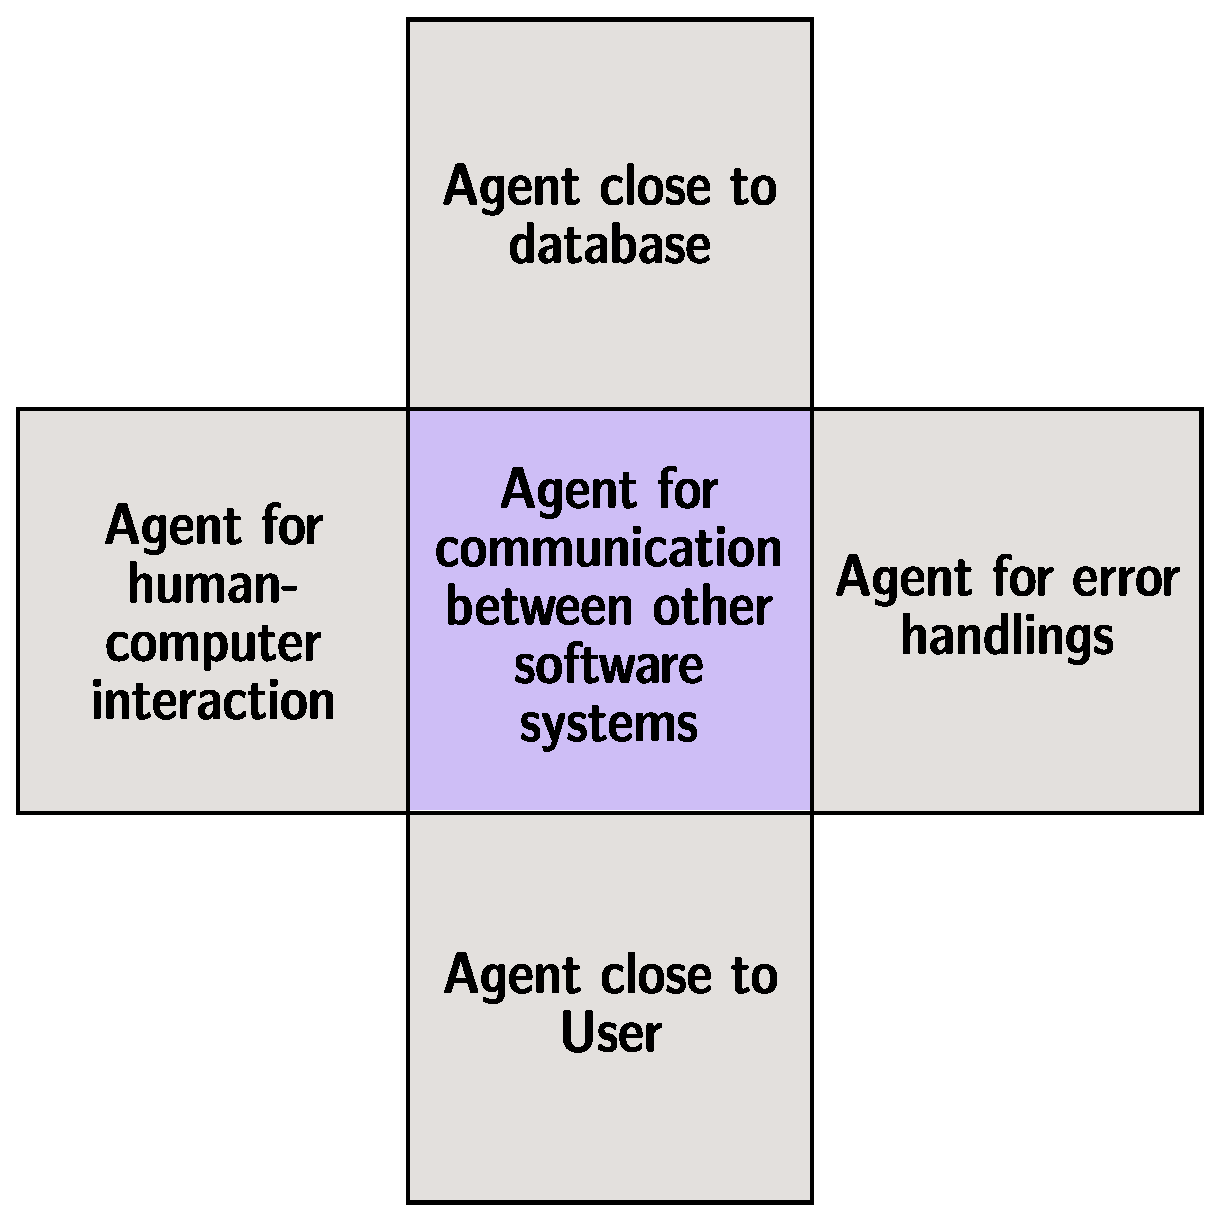
\includegraphics[width=0.4\textwidth]{./pics/problem.eps}\end{center}
 % problem.eps: 0x0 pixel, 300dpi, 0.00x0.00 cm, bb=0 -1 570 570

\end{multicols}

\section{Solution}

\section{Structure}	%Jaqueline

To provide the functionality of interactive software systems it is structured as a tree-like hierarchy of
PAC – agents. There are three types of agents (top-level agent, bottom-level agent and intermediate
agent), so “every agent is responsible for a specific aspect of the applications functionality” (cf.
Buschmann et al., Pattern-orientated software architecture: page 146). Agents have three
responsibilities: presentation (graphical user interface), abstract (data model) and control
(communication and mediation between agents).

\subsection{Top-Level Agent}	%Jaqueline

The top-level agent is unique in the system. He accepts all global responsibilities, such as the
database and parts of the user input – interfaces, that cannot be assigned to specific subtasks (cf.
Buschmann et al., Pattern-orientated software architecture: page 147).

The abstraction component of the top-level agent is the interface to all information about the data
model. This includes to manipulate and retrieve information about the data model.
The presentation component of the top-level agent has none, until only a few responsibilities. The
bottom-level agents resume the presentation.

The control component consists of three subcomponents. First, top-level agents allow access to data
model for lower-level agents. Second is the coordination of all PAC agents, to “ensure correct
collaboration and data exchange” (cf. Buschmann et al., Pattern-orientated software architecture:
page 149). Last, a subcomponent is to collect information about interaction between user and
system. The top-level agent checks, if a user request can be performed by data model and
documents history of operations done on the functional core.



\subsection{Bottom-Level Agent}



\subsection{Intermediate-Level Agent}

\begin{center}
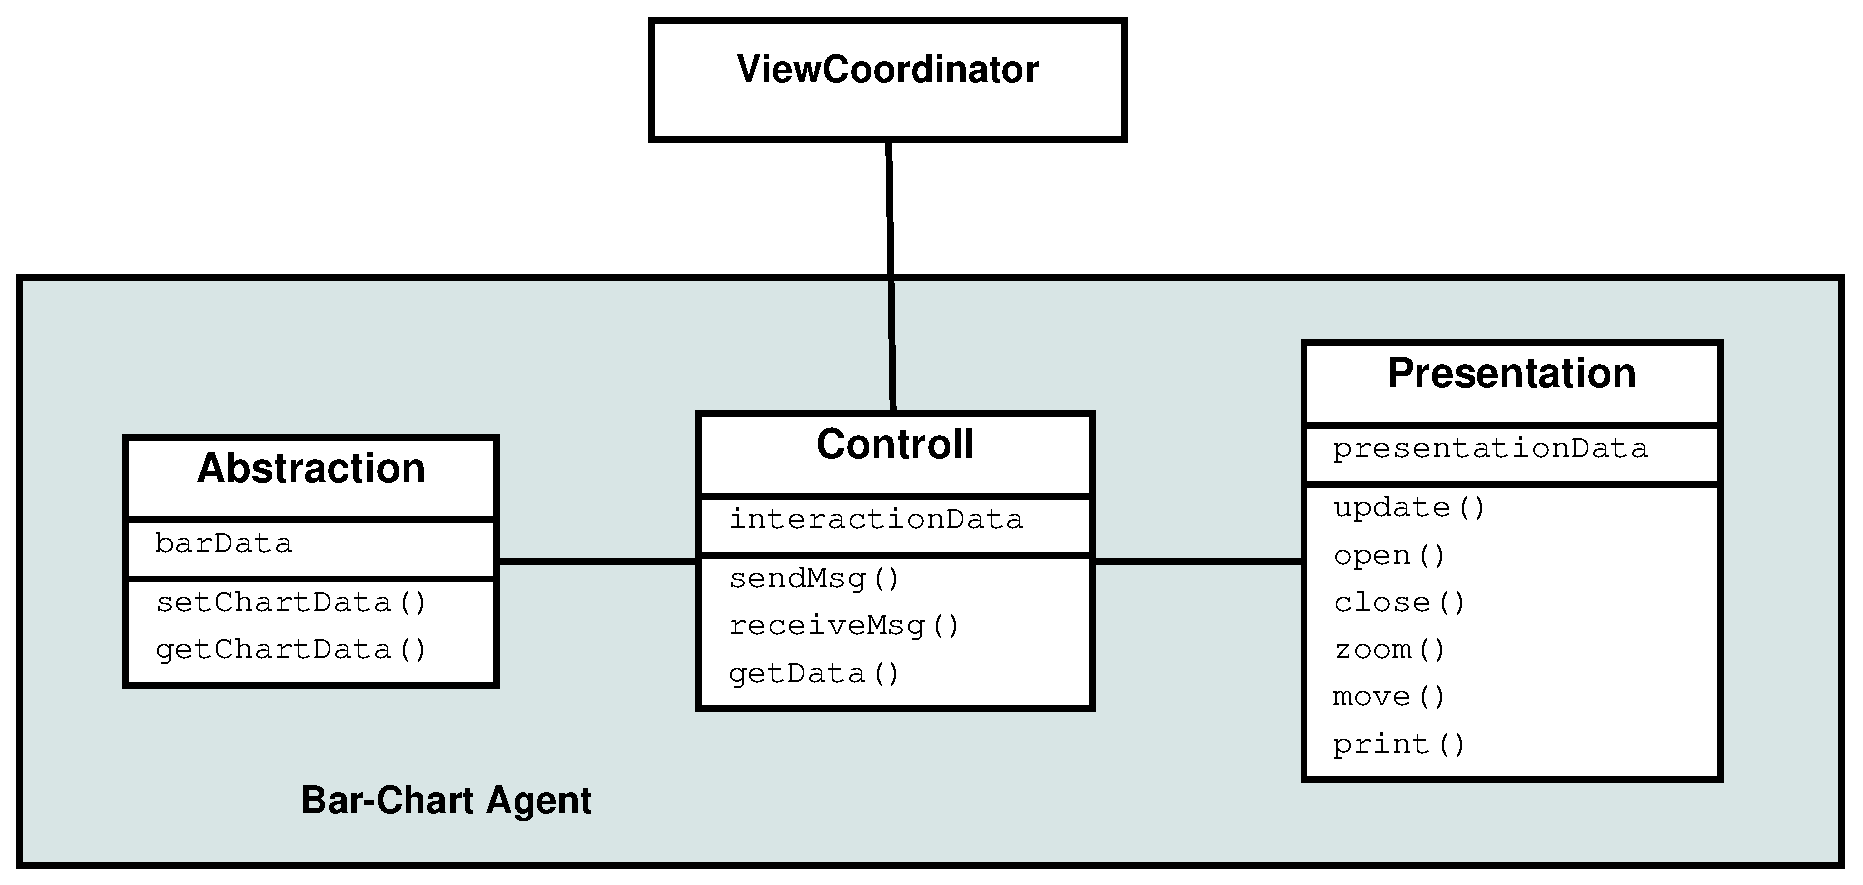
\includegraphics[width=.8\textwidth]{./pics/Components.eps}\end{center}
% Components.eps: 0x0 pixel, 300dpi, 0.00x0.00 cm, bb=0 0 878 409


The intermediate-level PAC agent is responsible for composition and coordination. The agent has to define new abstraction. The other job of the intermediate-level agent is to manage consistency steadiness between the different lower-level agents. 

The abstract component manages the data of the intermediate-level PAC agent. The user interface is implemented by the presentation component. The control component communicates with top-level and bottom-level agents. 

In the information system for political elections we need one intermediate-level agent. The presentation component of the agents creates a tool to view the election data for example in bar or pie charts.  The abstraction component is responsible for all currently active views. Each view is created by one bottom-level agent. The control component must control all subordinate agents. The intermediate-level agent informs the bottom-level agent about changes made by the top-level agent. The intermediate-level agent creates and deflects bottom-level agents on user request. 


\section{Dynamics}

Now we will take a deeper look at the internal functions of PAC, analysing two scenarios.  In the first one we describe what will happen, if a new bar-chart view of the election data is opened.
First a query is send to the presentation component of the view coordinator to open a new bar chart. Then the control of the view coordinator starts the required bar-chart agent. That means the view coordinator sends an open event to the control component of the bar chart agent. At next the control component of the bar chart gets the data from the top-level agent and saves it in the abstraction component. After the process is finished the control component can enable the presentation component to display the chart. At last the presentation component displays a new window with the retrieved data from its belonging abstraction component.

%Bild 1

In the second scenario we have entered new election data in the system.  At first the new data is entered in a spreadsheet and the control component of the spreadsheet agent sends it to the top-level agent. After receiving the spreadsheet the top-level abstraction is requested to change the repository. Then the top-level control component is asked to update all belonging agents with the new data. Therefor we need the view coordinator agent. The view coordinator sends to all view agents a change notification. Now all low-level Agents update their data.  

%Bild 2

\section{Known Uses}

%end Groups I and H

\section{Quellen}

%TODO Quellenangaben


\chapter{Microkernel}
\chapter{Reflection}

\end{document}
